\documentclass[11pt]{article}
\usepackage{geometry}                % See geometry.pdf to learn the layout options. There are lots.
\geometry{letterpaper}                   % ... or a4paper or a5paper or ... 
%\geometry{landscape}                % Activate for for rotated page geometry
%\usepackage[parfill]{parskip}    % Activate to begin paragraphs with an empty line rather than an indent
\usepackage{graphicx}
\usepackage{amssymb}
\usepackage{slashed}
\usepackage{epstopdf}
\usepackage{amsmath}
\usepackage{listings}
\DeclareGraphicsRule{.tif}{png}{.png}{`convert #1 `dirname #1`/`basename #1 .tif`.png}

\graphicspath{ {Figures/} }

\usepackage{lmodern}

\usepackage{mmacells}


\mmaDefineMathReplacement[?]{<=}{\leq}
\mmaDefineMathReplacement[?]{>=}{\geq}
\mmaDefineMathReplacement[?]{!=}{\neq}
\mmaDefineMathReplacement[?]{->}{\to}[2]
\mmaDefineMathReplacement[?]{:>}{:\hspace{-.2em}\to}[2]
\mmaDefineMathReplacement{?}{\notin}
\mmaDefineMathReplacement{?}{\infty}
\mmaDefineMathReplacement{??}{\mathbbm{d}}


\mmaSet{
  morefv={gobble=2},
  linklocaluri=mma/symbol/definition:#1,
  morecellgraphics={yoffset=1.9ex}
}

\setlength{\parindent}{0pt}
\newcommand{\mychi}{\raisebox{0pt}[1ex][1ex]{$\chi$}}
\def\sp{\slashed{p}}
\def\sk{\slashed{k}}
\def\cn{\mychi^0}
\def\cp{\mychi^+}
\def\cm{\mychi^-}
\def\cpp{\mychi^{++}}
\def\cmm{\mychi^{--}}
\def\gm{\gamma^{\mu}}
\def\gn{\gamma^{\nu}}
\def\gp{\gamma^{\rho}}
\def\km{k_{\mu}}
\def\kn{k_{\nu}}
\def\kp{k_{\rho}}
\def\Mp{M_{\text{pole}}}
\def\Mpa{M_{\text{pole},A}}
\def\Mpb{M_{\text{pole},B}}
\renewcommand{\d}{\ensuremath{\operatorname{d}\!}}
\def\kmpm{k^{\mu}p_{\mu}}
\def\he{\frac{\epsilon}{2}}

\newcommand{\mb}{\textsf{Mass Builder} \! }
\newcommand{\tsil}{\textsf{TSIL} \! }
\newcommand{\tarcer}{\textsf{TARCER} \! }


\begin{document}
%\maketitle
\today\\

In the following I use bold-face for the divergent integrals and normal type for the finite pieces, as defined in the TSIL manual.  I use $\tt{TAI}$ to refer to TARCER notation and $A$ for TSIL notation as there is a different normalisation between such integrals.  We define $\kappa = 1/16\pi^2$.

The field theory we will deal with here is that with Lagrangian
\begin{align}
\mathcal{L} = -\frac{1}{2}m^2s^2-\frac{g}{3!}s^3-\frac{\lambda}{4!}s^4
\end{align}


\section{One-loop self energy}
\begin{figure}[h!]
\center
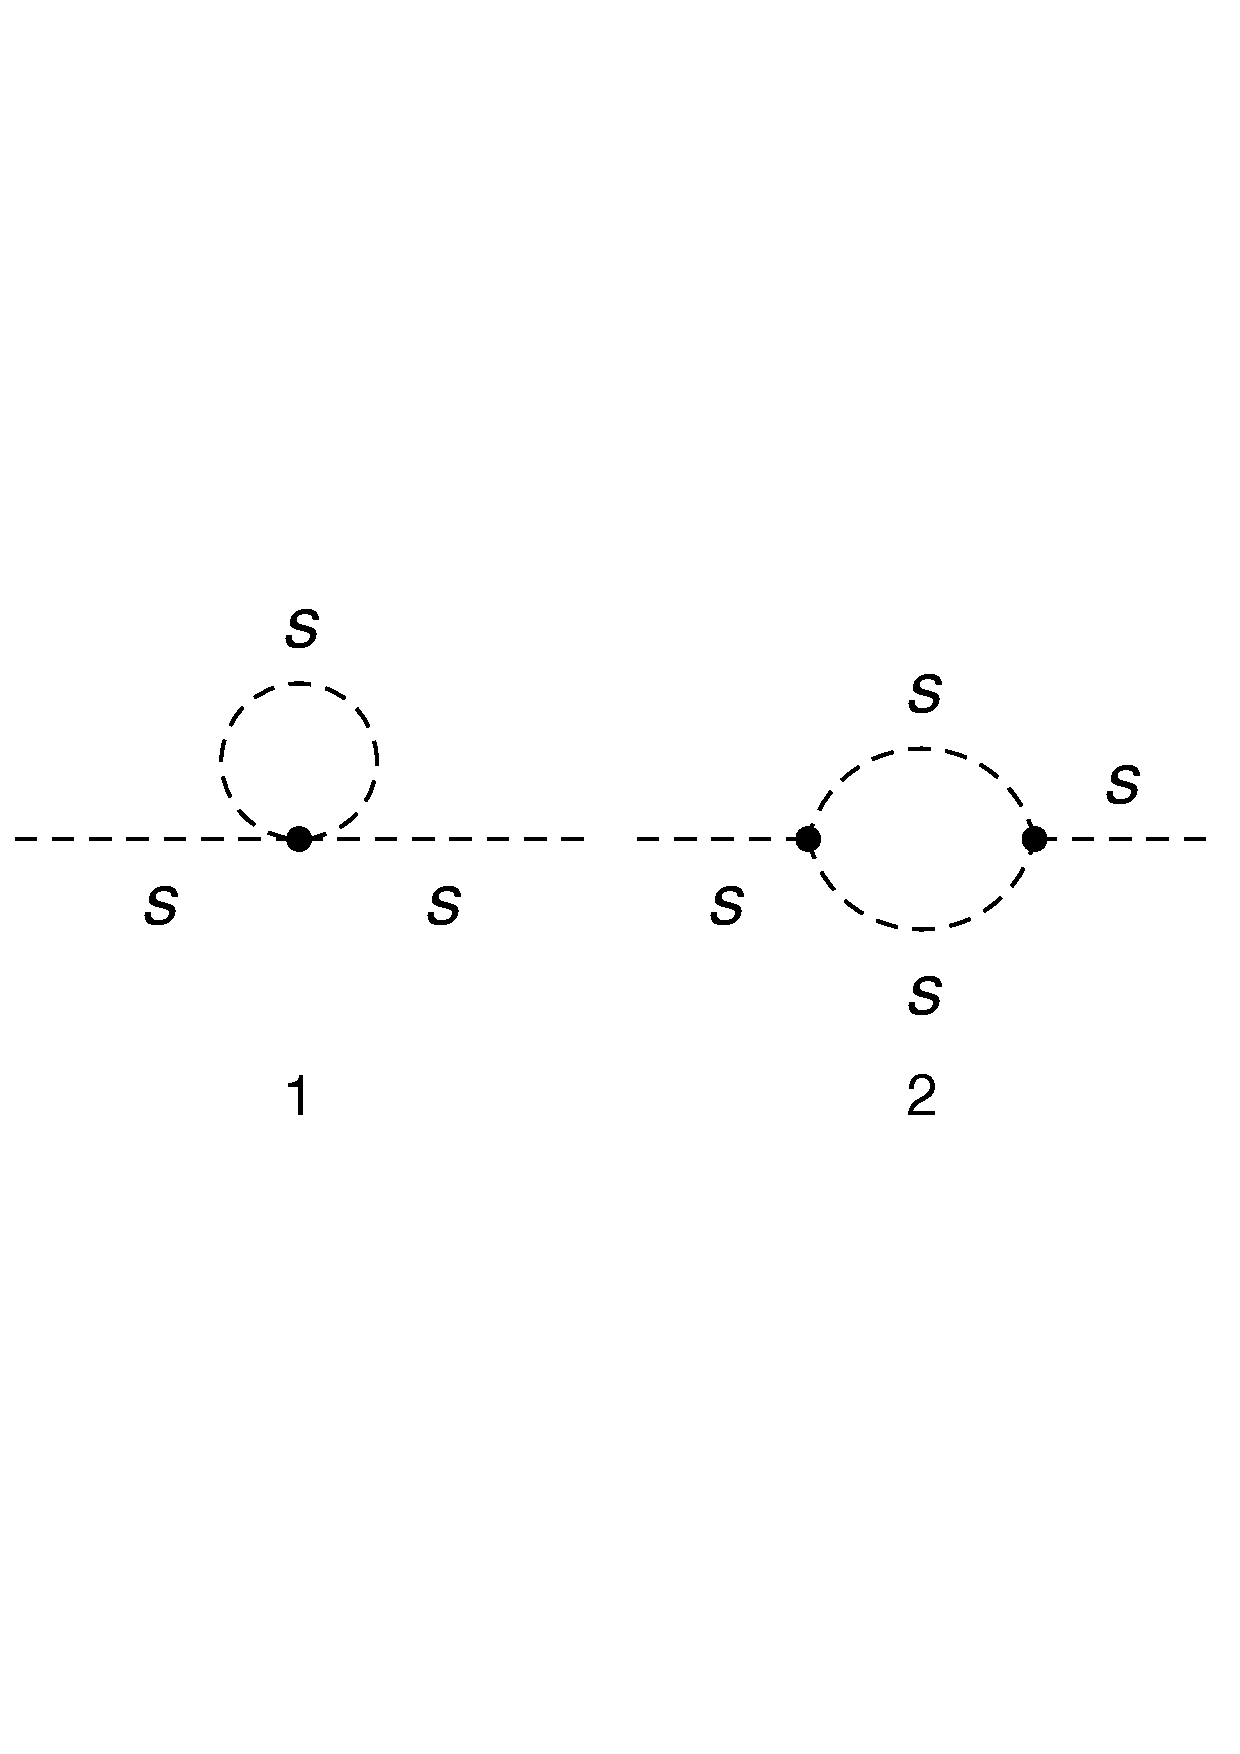
\includegraphics[width=0.6\textwidth]{1loop.pdf}\\
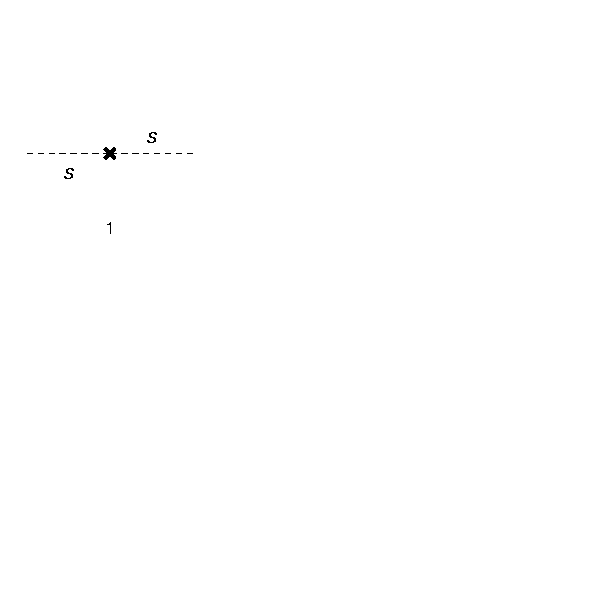
\includegraphics[width=0.3\textwidth]{1loop_1c.pdf}
\caption{The one-loop order loop (\textit{top}) and counter-term (\textit{bottom}) corrections to the scalar propagator.}\label{fig:1loop}
\end{figure}

The scalar propagator has two loop corrections and one counter-term correction at the one-loop order which are represented in Figure \ref{fig:1loop} top and bottom respectively.  Although these are easily written down by hand we use \mb to carry out the calculation and demonstrate where we need to account for sign differences between the computational tools we interface with.

The amplitudes from the loop corrections as output from \tarcer are
\begin{align}
\Pi^{(1)}_1 = -i \kappa \frac{\lambda}{2} \mathbf{TAI}(m^2)
\end{align}
and
\begin{align}
\Pi^{(1)}_2 =-i \kappa \frac{g^2}{2} \mathbf{TBI}(m^2,m^2)
\end{align}
first we must account for an overall negative sign in the amplitude, and then use the relationship $i\mathbf{TAI} = \mathbf{A}$ and $-i\mathbf{TBI} = \mathbf{B}$ to convert to \tsil notation
\begin{align}
\Pi^{(1)}_1 = \kappa \frac{\lambda}{2} \mathbf{A}(m^2)
\end{align}
and
\begin{align}
\Pi^{(1)}_2 = -\kappa \frac{g^2}{2} \mathbf{B}(m^2,m^2).
\end{align}

The counter-term diagram is trivial to calculate by hand, yet again we will take the result from \tarcer which is
\begin{align}
\Pi^{(1c)}_1 =  -d_1
\end{align}
so again we need to make a sign change and obtain
\begin{align}
\Pi^{(1c)}_1=  d_1.
\end{align}


We can now determine this counter-term coupling from a simple calculation at one-loop, which we must do by hand.  The full one-loop self energy, including counter-terms, is
 \begin{align}
 \Pi_1 = \frac{1}{2}\kappa\lambda\left(A(m^2)+\epsilon A_{\epsilon}(m^2)-\frac{m^2}{\epsilon}\right)- \frac{1}{2}\kappa g^2\left(B(m^2)+\epsilon B_{\epsilon}(m^2)+\frac{1}{\epsilon}\right)+d_1
 \end{align}
so the divergent part is
\begin{align}
\Pi_1^{1/\epsilon}=  -\frac{1}{2\epsilon}\kappa\left(\lambda m^2+g^2\right)+d_1
\end{align}
so we find
\begin{align}
d_1=\frac{\kappa}{2\epsilon} \left(g^2+\lambda m^2\right)+\mathcal{O}(\kappa^2)
\end{align}
where we allow for high order terms which are required to cancel divergences from amplitudes above the one-loop order.  This counter-term is all we will need to compute the finite piece of the self energy at two-loop order under certain assumptions.

So at the one-loop level we make one sign change to the \tarcer output to be able to compute the self energy correctly via the \tsil integrals.

\section{Two-loop self energy}

There are 9 loop corrections and 5 counter-term corrections to the scalar propagator at the two-loop level.  We present the results as output by \tarcer and the required conversions to \tsil integrals on a diagram by diagram basis in this section.

\subsection*{Diagram 1}
\begin{center}
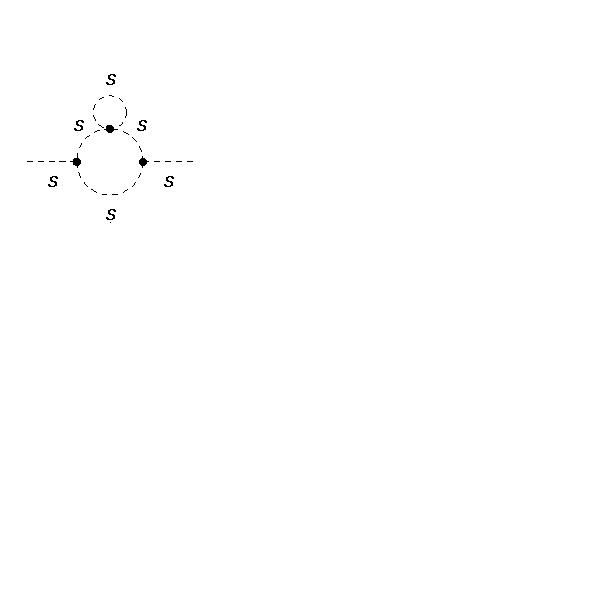
\includegraphics{2loop_1.pdf}\\
\end{center}
This digram is given by \tarcer to be
\begin{align}
\Pi^{(2)}_1 = \kappa^2\frac{g^2\lambda}{4} \frac{  \mathbf{TAI}(m^2) \left[ 2(D-3)m^2\mathbf{TBI}(m^2,m^2) - (D-2) \mathbf{TAI}(m^2) \right] }{m^2 (4m^2-p^2) }
\end{align}
so after accounting for the negative sign, and converting to TSIL notation (which also introduces a negative sign, due to the two factors of $i$) we obtain
\begin{align}
\Pi^{(2)}_1 = \kappa^2\frac{g^2\lambda}{4} \frac{  \mathbf{A}(m^2) \left[ -2(D-3)m^2\mathbf{B}(m^2,m^2) - (D-2) \mathbf{A}(m^2) \right] }{m^2 (4m^2-p^2) }
\end{align}


\subsection*{Diagram 2 and 3}
\begin{center}
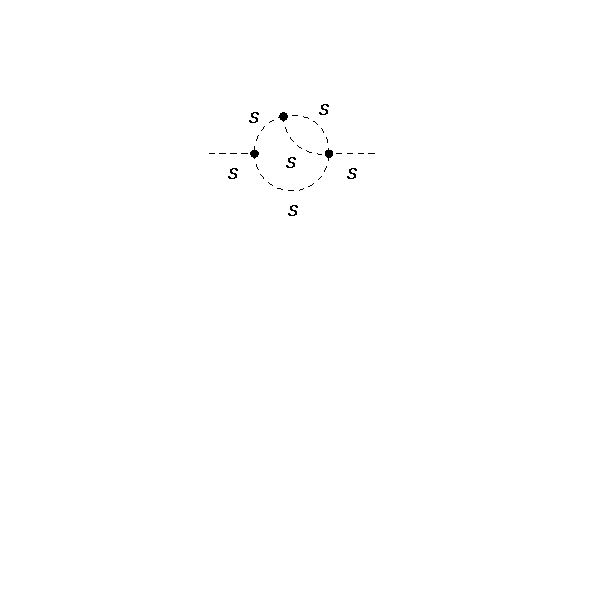
\includegraphics{2loop_2.pdf}\ \ \ \ \ \ 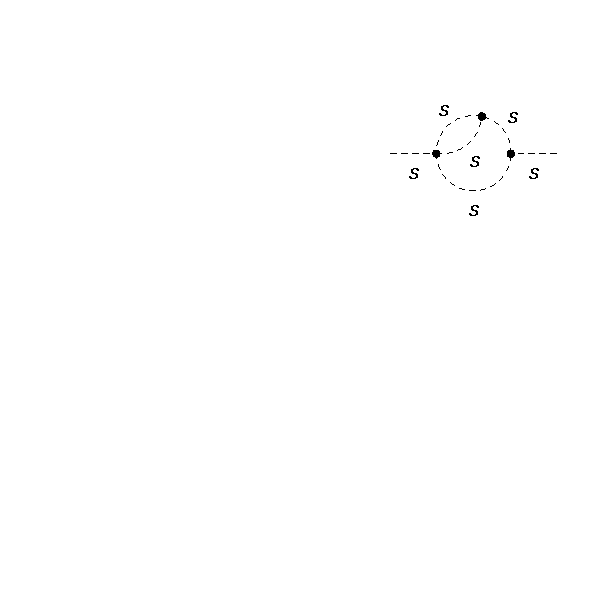
\includegraphics{2loop_3.pdf}\\
\end{center}
Diagrams 2 and 3 are identical and are given in \tarcer to be
\begin{align}
\Pi_2 = \kappa^2 \frac{g^2\lambda}{2} \mathbf{TVI}(m^2,m^2,m^2,m^2)
\end{align}
so combining these together and using the result $ \mathbf{TVI}=-\mathbf{U}$ we obtain, after including the sign change, the same result as we could get by simply looking at the topology of the diagram
\begin{align}
\Pi_2 =  \kappa^2 g^2\lambda \mathbf{U}(m^2,m^2,m^2,m^2).
\end{align}



\subsection*{Diagram 4}
\begin{center}
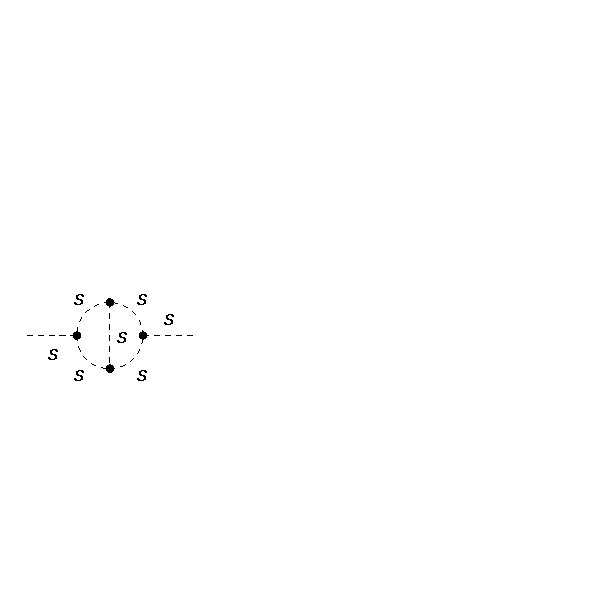
\includegraphics{2loop_4.pdf}
\end{center}
\begin{align}
\Pi_4 = \kappa^2 \frac{g^4}{2} \mathbf{TFI}(m^2,m^2,m^2,m^2,m^2)
\end{align}

Accounting for the negative sign and using the relationship $\mathbf{TFI}=\mathbf{M}$ we obtain the same result as the notes
\begin{align}
\Pi_4 = - \kappa^2 \frac{g^4}{2} \mathbf{M}(m^2,m^2,m^2,m^2,m^2)
\end{align}

\subsection*{Diagram 5}
\begin{center}
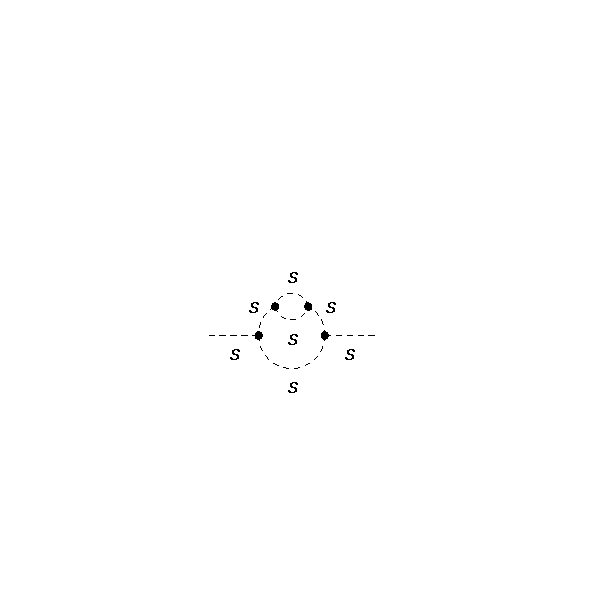
\includegraphics{2loop_5.pdf}
This diagram is given by TARCER to be after full reduction

\end{center}
\begin{align}
\begin{split}
\Pi_5 =& \kappa^2 \frac{g^4}{12 m^4} \left( \frac{3(3D-8)m^2(2m^2-p^2)}{p^2(4m^2-p^2)}\mathbf{TJI}(m^2,m^2,m^2)\right. \\
&+ \frac{4m^2(m^2-p^2)(9m^2-p^2)}{p^2(4m^2-p^2)}\mathbf{TJI}_2(m^2,m^2,m^2)\\
&+\frac{3(D-2)m^2(2m^2-p^2)}{p^2(4m^2-p^2)}\mathbf{TKI}(m^2,m^2,m^2)\\
&+\frac{m^2(D p^2+2(D-9)m^2)}{4m^2-p^2}\mathbf{TVI}(m^2,m^2,m^2,m^2)\\
&\left.+2(D-2)\mathbf{TAI}(m^2) \mathbf{TBI}(m^2,m^2) \right)
\end{split}
\end{align}
accounting for the negative sign and converting to TSIL notation we obtain

\begin{align}
\begin{split}
\Pi_5 =& - \kappa^2 \frac{g^4}{12 m^4} \left( \frac{3(3D-8)m^2(2m^2-p^2)}{p^2(4m^2-p^2)}\mathbf{S}(m^2,m^2,m^2)\right. \\
&-\frac{4m^2(m^2-p^2)(9m^2-p^2)}{p^2(4m^2-p^2)}\mathbf{T}(m^2,m^2,m^2)\\
&+\frac{3(D-2)m^2(2m^2-p^2)}{p^2(4m^2-p^2)}\mathbf{I}(m^2,m^2,m^2)\\
&-\frac{m^2(D p^2+2(D-9)m^2)}{4m^2-p^2}\mathbf{U}(m^2,m^2,m^2,m^2)\\
&\left.+2(D-2)\mathbf{A}(m^2) \mathbf{B}(m^2,m^2) \right)
\end{split}
\end{align}


\subsection*{Diagram 6}
\begin{center}
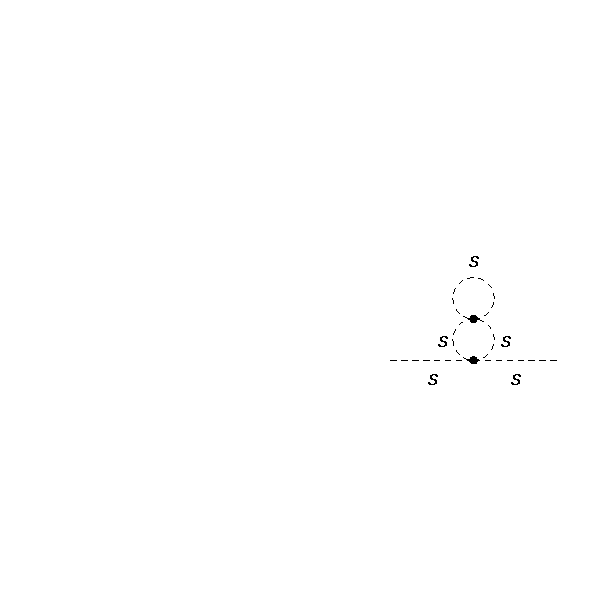
\includegraphics{2loop_6.pdf}
\end{center}
This diagram is given by TARCER to be
\begin{align}
\Pi_6 &= \kappa^2 \frac{\lambda^2(D-2)}{8}\frac{ \left({\tt{\mathbf{TAI}}} (m^2)\right)^2}{ m^2 }  
\end{align}
converting to TSIL notation and accounting for the negative sign we obtain
\begin{align}
\Pi_6 &= \kappa^2 \frac{\lambda^2(D-2)}{8}\frac{ \left({\tt{\mathbf{A}}} (m^2)\right)^2}{ m^2 }  
\end{align}

now we must set $D=4-r\epsilon$ and account for finite contributions which come from the divergent parts of the basis integrals.  I leave the factor of $r$ in for now.  The basis integrals can be expressed as a finite piece plus a divergent piece, so we have
\begin{align}
{\tt{\mathbf{TAI}}}(x) &= \frac{ix}{\epsilon} +  {\tt{TAI}}(x)
\end{align}
where we have converted \textcolor{blue}{(1.28)} of the TSIL manual into the TARCER definition using $\mathbf{A}= ia \tt{\mathbf{TAI}}$ and taking $a=1$ for small $\epsilon$ \footnote{I have tried keeping these additional $\epsilon$ terms in here coming from the $a$ factor, but I have found it leads to only more problems and additional terms which don't make sense to me.  Although I'm still a little uncertain, I have convinced myself taking $\epsilon \rightarrow 0$ for converting between these different normalisations is okay in this context.}.  So the amplitude becomes
\begin{align*}
\Pi_1 &= \frac{\lambda^2(2-r\epsilon)}{8 m^2 }       \left( {\tt{TAI}}(m^2) +\frac{im^2}{\epsilon}\right)^2  \\
&= \frac{\lambda^2}{4 m^2 }  {\tt{TAI}}(m^2) \left( \frac{ {\tt{TAI}}(m^2) } {m^2} - ir\right)
\end{align*}
where we ignore any divergent terms (assuming these will be cancelled by the counter-terms) and take the limit of $\epsilon\rightarrow 0$.
Finally we need to evaluate this in terms of TSIL integrals, which have a different normalization.  The relationship is $\mathbf{A}= ia \tt{\mathbf{TAI}}$ where $a = (4\pi\mu^2)^{2-D/2} \approx 1 +\frac{r\epsilon}{2}\log(4\pi\mu^2)+\mathcal{O}(\epsilon^2)$.  Since we have already removed the divergent parts and are dealing with finite integrals, I take $\epsilon =  0$ and we simply have $\mathbf{A}= i \tt{\mathbf{TAI}}$.  Therefore we end up with, after setting $r=2$ and taking account for the negative sign as with all other integrals,
\begin{align}
\Pi_1 & = \kappa^2  \frac{\lambda^2}{4 } A(m^2) \left( \frac{A(m^2)}{m^2} + 2 \right)
\end{align}




\subsection*{Diagram 7}
\begin{center}
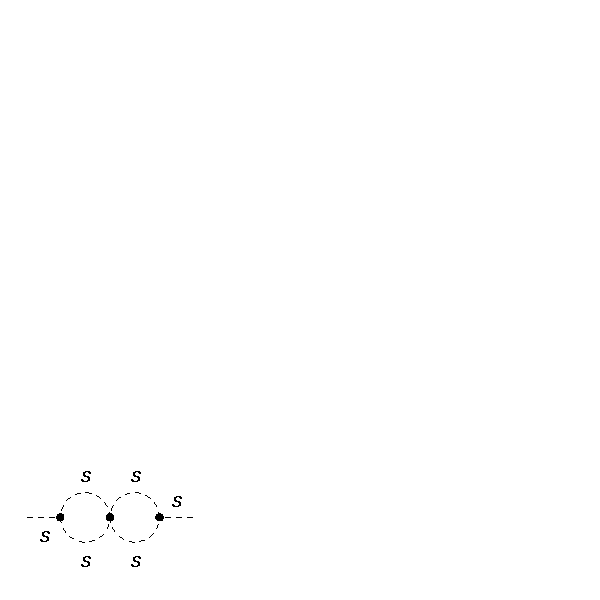
\includegraphics{2loop_7.pdf}
\end{center}
This diagram is given by TARCER to be
\begin{align}
\Pi_7 & =  \kappa^2 \frac{g^2 \lambda}{4 } \left(\mathbf{TBI}(m^2,m^2)\right)^2
\end{align}
accounting for negative sign and using $-i\mathbf{TBI} = \mathbf{B}$ we obtain
\begin{align}
\Pi_7 & = \kappa^2 \frac{g^2 \lambda}{4 } \left(\mathbf{B}(m^2,m^2)\right)^2
\end{align}


\subsection*{Diagram 8}
\begin{center}
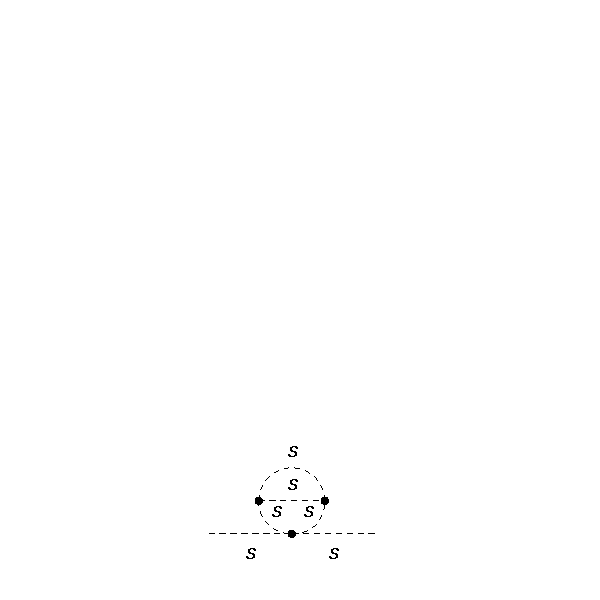
\includegraphics{2loop_8.pdf}
\end{center}
This diagram is given by TARCER to be
\begin{align}
\Pi_8 & = - \kappa^2\frac{g^2 \lambda}{12 m^2 } (D-3) \mathbf{TKI}(m^2,m^2,m^2)
\end{align}
converting to TSIL notation and accounting for the negative sign
\begin{align}
\Pi_8 & =  \kappa^2\frac{g^2 \lambda}{12 m^2 } (D-3) \mathbf{I}(m^2,m^2,m^2)
\end{align}
but we need another negative sign for the definition of K (apparently, check this)
\begin{align}
\Pi_8 & =  -\kappa^2\frac{g^2 \lambda}{12 m^2 } (D-3) \mathbf{I}(m^2,m^2,m^2)
\end{align}

\subsection*{Diagram 9}
\begin{center}
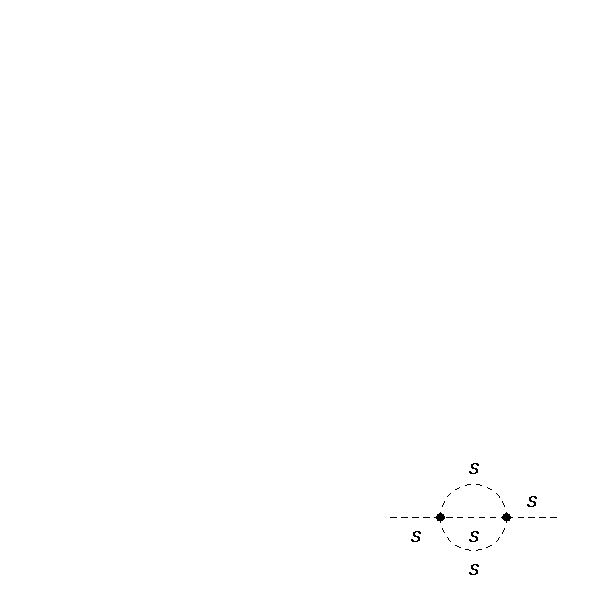
\includegraphics{2loop_9.pdf}
\end{center}
This diagram is given by TARCER to be

 \begin{align}
 \Pi_9 =\kappa^2 \frac{\lambda^2 {\tt{\mathbf{TJI}}}(m^2,m^2,m^2) }{6}
 \end{align}
 where ${\tt{\mathbf{TJI}}} = {\tt{\mathbf{TJI}}}\{1,1,1\}$ which is equivalent to the TSIL integral $S(x,y,z)$ for $a=1$, accounting for the negative sign we obtain
 \begin{align*}
 \Pi_9 & = -\kappa^2\frac{\lambda^2}{6}\textbf{S}(m^2,m^2,m^2)
 \end{align*}
 
 
 
 \section*{Counter-terms}
 
 
 The two-loop order counter-terms cancel divergences from the loop corrections and provide finite contributions to the total self energy.  In the MS bar scheme the counter-term couplings are of at least first order in $\mathcal{O}(1/\epsilon)$, so we can identify which counter-term diagrams will contribute finite contributions.
 
 
 
 
 \subsection*{Counter-diagram 1}
\begin{center}
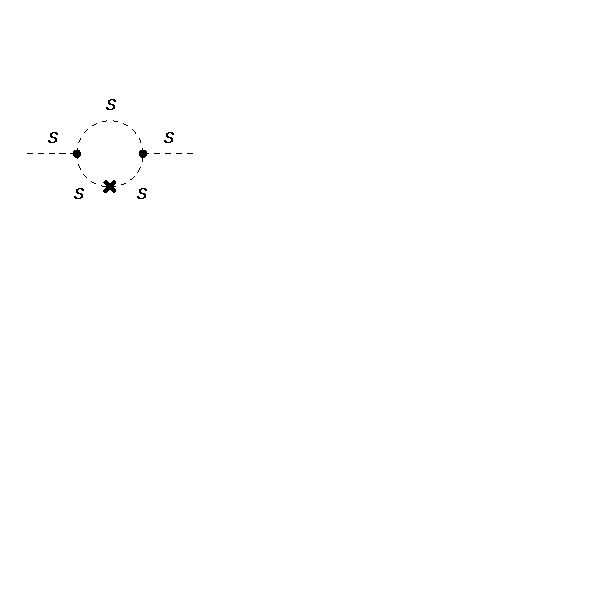
\includegraphics{2loop_1c.pdf}
\end{center}
 
 \begin{align}
 \Pi_1 = \kappa \frac{i  d_1 g^2}{ 2 m^2 (4m^2-p^2)} \left( (D-2){\tt{\mathbf{TAI}}}(m^2)-2(D-3){\tt{\mathbf{TBI}}}(m^2,m^2) \right)  
 \end{align}
 
 converting to TSIL notation, accounting for the negative sign and multiplying by $1/\epsilon$ we obtain
  \begin{align}
 \Pi_1 = \kappa \frac{ d_1 }{\epsilon}\frac{g^2}{ 2 m^2 (4m^2-p^2)} \left( (2-2\epsilon){\tt{\mathbf{A}}}(m^2)+2(1-2\epsilon){\tt{\mathbf{B}}}(m^2,m^2) \right)  
 \end{align}
 from which we obtain the finite contributions
\begin{align}
 \Pi_1 = \kappa d_1 \frac{g^2}{ 2 m^2 (4m^2-p^2)} \left( -2 A(m^2)+2A_{\epsilon}(m^2)-4m^2B(m^2,m^2)+2Bm^2_{\epsilon}(m^2,m^2)\right)
 \end{align}
 
  \subsection*{Counter-diagram 2}
 \begin{center}
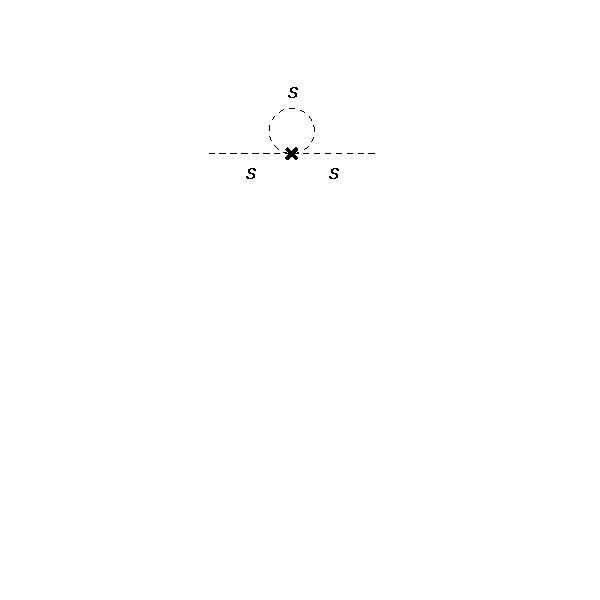
\includegraphics{2loop_2c.pdf}
\end{center}

 \begin{align}
 \Pi_2 = - \kappa i  \frac{d_{\lambda}}{2} {\tt{\mathbf{TAI}}}(m^2)
 \end{align}
 which after accounting for the negative sign and converting from TARCER to TSIL we obtain
  \begin{align}
 \Pi_2 = - \kappa \frac{d_{\lambda}}{2} \ {\tt{\mathbf{A}}}(m^2)
 \end{align}
 
   \subsection*{Counter-diagram 3 and 5}
 \begin{center}
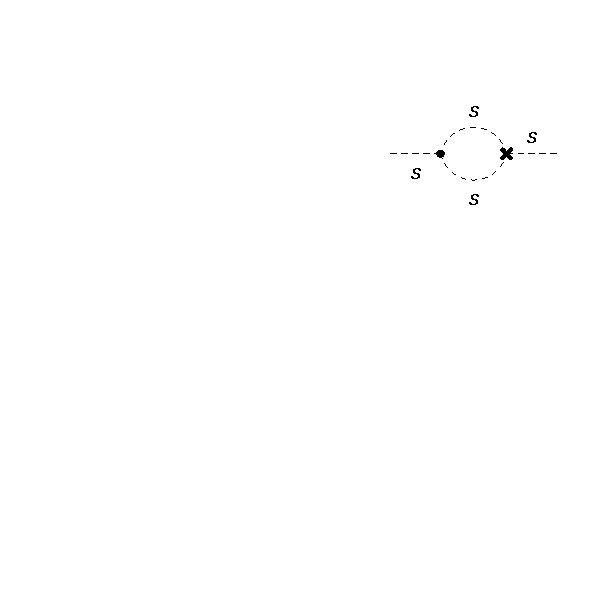
\includegraphics{2loop_3c.pdf} \ \ \ \ \ \ \ 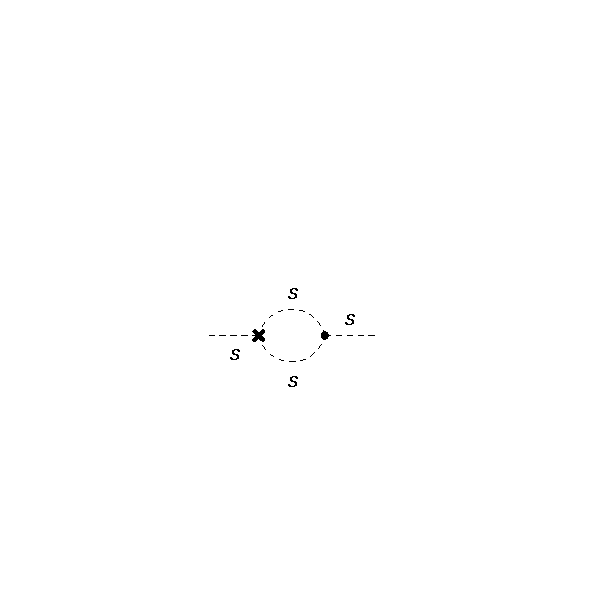
\includegraphics{2loop_5c.pdf}
\end{center}

 \begin{align}
 \Pi_{3,5} = - \kappa i \frac{g d_g}{2} {\tt{\mathbf{TBI}}}(m^2,m^2) 
 \end{align}
  
Combining these together and accounting for the negative sign we obtain
 \begin{align}
 \Pi_{3,5} = i \kappa g d_g {\tt{\mathbf{TBI}}}(m^2,m^2) 
 \end{align}
converting to TSIL notation and inserting the counter-term coupling (each introduces a negative sign)
\begin{align}
 \Pi_{3,5} = \kappa^2 g \frac{c_{1,1}^g}{\epsilon} {\tt{\mathbf{B}}}(m^2,m^2) 
 \end{align}

 
\subsection*{Counter-diagram 4}
\begin{center}
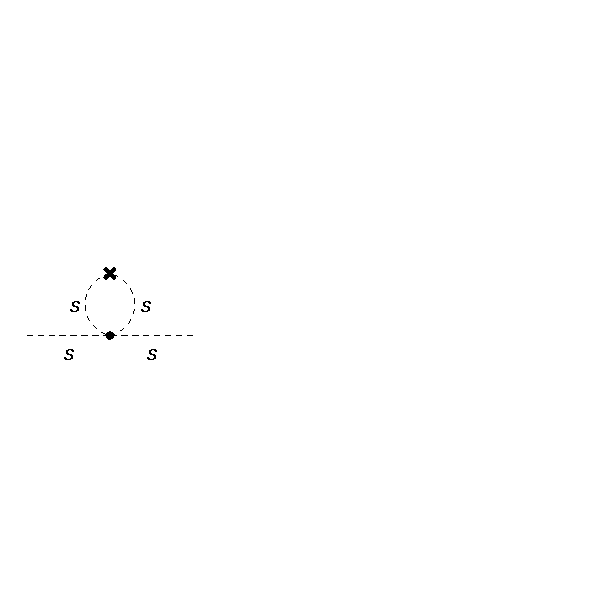
\includegraphics{2loop_4c.pdf}
\end{center}

 \begin{align}
 \Pi_4 =  \kappa \frac{-i \lambda d_1 (D-2)}{ 4 m^2} {\tt{\mathbf{TAI}}}(m^2) 
 \end{align}
 
 accounting for the negative sign and changing notation we obtain
 \begin{align}
 \Pi_4 =  \kappa \frac{ \lambda d_1 (D-2)}{ 4 m^2} {\tt{\mathbf{A}}}(m^2) 
 \end{align}
 
 


 \section*{Comments}
 
 In Stephen's working the $A_{\epsilon}(x')$ terms cancel between the diagrams and the counter-term diagrams.  However,
 
 \begin{align*}
 A_{\epsilon}(x') = \frac{A_{\epsilon}(x)}{x}-\frac{A(x)}{x}
 \end{align*}
 
 so there is actually a $A(x)$ term here that is cancelling out between the normal diagrams and the finite contribution from the counter-terms, but it's kind of hidden.  In our approach, we do not invoke this derivative at all (and don't carry around non-expanded things like  $A_{\epsilon}(x')$ ) , and thus our diagram (diagram 5) explicitly contains this $A(x)$ term, so it appears wrong until we actually consider the counter-term.  In Stephen's approach we could actually just ignore the  $A_{\epsilon}(x')$  term from the beginning knowing it will cancel.  All this only becomes apparent when we expand out  $A_{\epsilon}(x')$ and look at the counter-term and normal diagrams separately.
 
 
 
 
 
 
 
 
 \end{document}  